\subsection{Further analysis}
In this section, we illustrate ablation studies, failure cases and timings of our methods.

\begin{table}[t]
\tablestyle{1.5pt}{1.2}
\begin{tabular}{l|x{16}x{16}|x{32}|x{22}x{22}|x{32}}

		& \texttt{AN}& \texttt{RN} & \texttt{EAO} $\uparrow$ & $\mathcal{J}_{\mathcal{M}\uparrow}$ & $\mathcal{F}_{\mathcal{M}\uparrow}$   & \texttt{Speed} \\[.1em]
\shline
SiamFC             & \cmark  &                   & 0.188   & -             & -             & 86    \\
SiamFC             &         & \cmark            & 0.251   & -             & -             & 40    \\
SiamRPN            & \cmark  &                   & 0.243   & -             & -             & \textbf{200}   \\
SiamRPN            &         & \cmark            & 0.359   & -             & -             & 76    \\ \hline 
SiamMask-2B w/o R        &         & \cmark            & 0.326   & 62.3          & 55.6          & 43    \\
SiamMask w/o R        &         & \cmark            & 0.375   & 68.6          & 57.8          & 58 \\ \hline
SiamMask-2B-score        &         & \cmark            & 0.265   & -             & -             & 40    \\
SiamMask-box        &         & \cmark            &  0.363   & -             & -             & 76    \\ \hline 
SiamMask-2B       &         & \cmark            & 0.334   & 67.4          & 63.5          & 60    \\
SiamMask       &         & \cmark            & \textbf{0.380} & \textbf{71.7} & \textbf{67.8} & 55    \\ 
\end{tabular}
\vspace{1mm}
\caption{Ablation studies on VOT-2018 and DAVIS-2016.}
\label{tab:arch}
\end{table}


\mypar{Network architecture.}
In Table~\ref{tab:arch}, \texttt{AN} and \texttt{RN} denote whether we use AlexNet or ResNet-50 as the shared backbone $f_{\theta}$ (Figure~\ref{fig:schematic}), while with ``w/o R'' we mean that the method does \emph{not} use  the refinement strategy of Pinheiro \etal~\cite{SharpMask}.
From the results of Table~\ref{tab:arch}, it is possible to make several observations.
(1) The first set of rows shows that, by simply updating the architecture of $f_{\theta}$, it is possible to achieve an important performance improvement.
However, this comes at the cost of speed, especially for SiamRPN.
(2) SiamMask-2B and SiamMask considerably improve over their baselines (with same $f_{\theta}$) SiamFC and SiamRPN.
(3) Interestingly, the refinement approach of Pinheiro \etal~\cite{SharpMask} is very important for the contour accuracy $\mathcal{F}_{\mathcal{M}}$, but less so for the other metrics.

\mypar{Multi-task training.}
We conducted two further experiments to disentangle the effect of multi-task training.
Results are reported in Table~\ref{tab:arch}.
To achieve this, we modified the two variants of SiamMask during inference so that, respectively, they report an axis-aligned bounding box from the score branch (SiamMask-2B-score) or the box branch (SiamMask-box).
Therefore, despite having been trained, the mask branch is \emph{not} used during inference.
We can observe how both variants obtain a modest but meaningful improvement with respect to their counterparts (SiamFC and SiamRPN): from 0.251 to 0.265 EAO for the \emph{two-branch} and from 0.359 to 0.363 for the \emph{three-branch} on VOT2018.

\mypar{Timing.} 
SiamMask operates online without any adaptation to the test sequence.
On a single NVIDIA RTX 2080 GPU, we measured an average speed of 55 and 60 frames per second, respectively for the \emph{two-branch} and \emph{three-branch} variants.
Note that the highest computational burden comes from the feature extractor $f_{\theta}$.

\begin{figure}[t]
\centering
\setlength{\tabcolsep}{0.25ex}

\begin{tabular}
{c cccc}
& 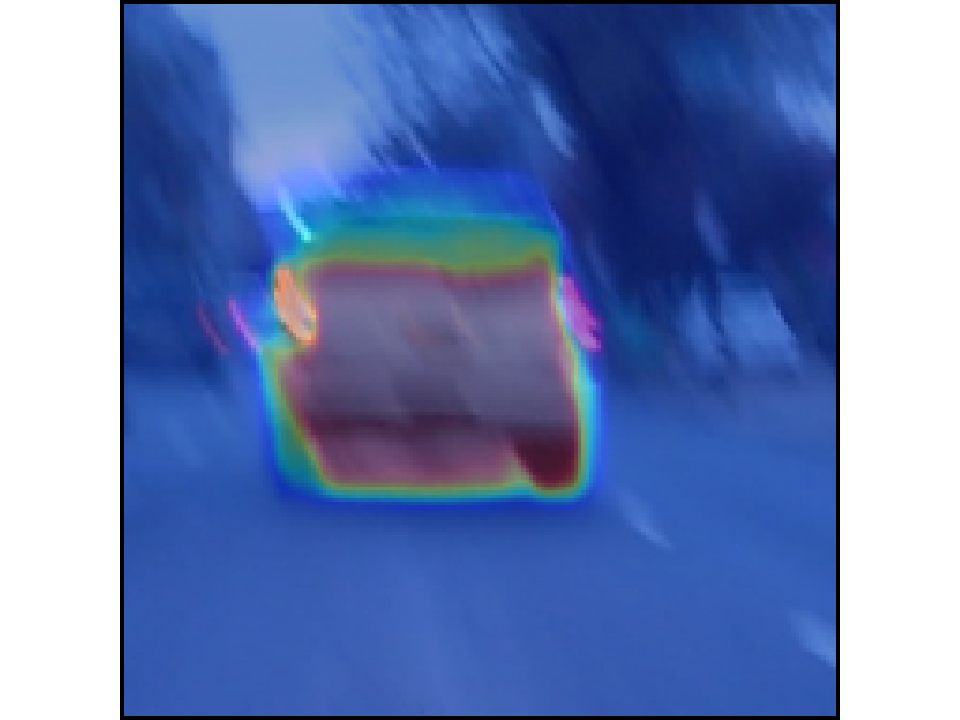
\includegraphics[trim={2cm 0cm 2cm 0cm},clip,height = 1in]{img/fail/03249}
& 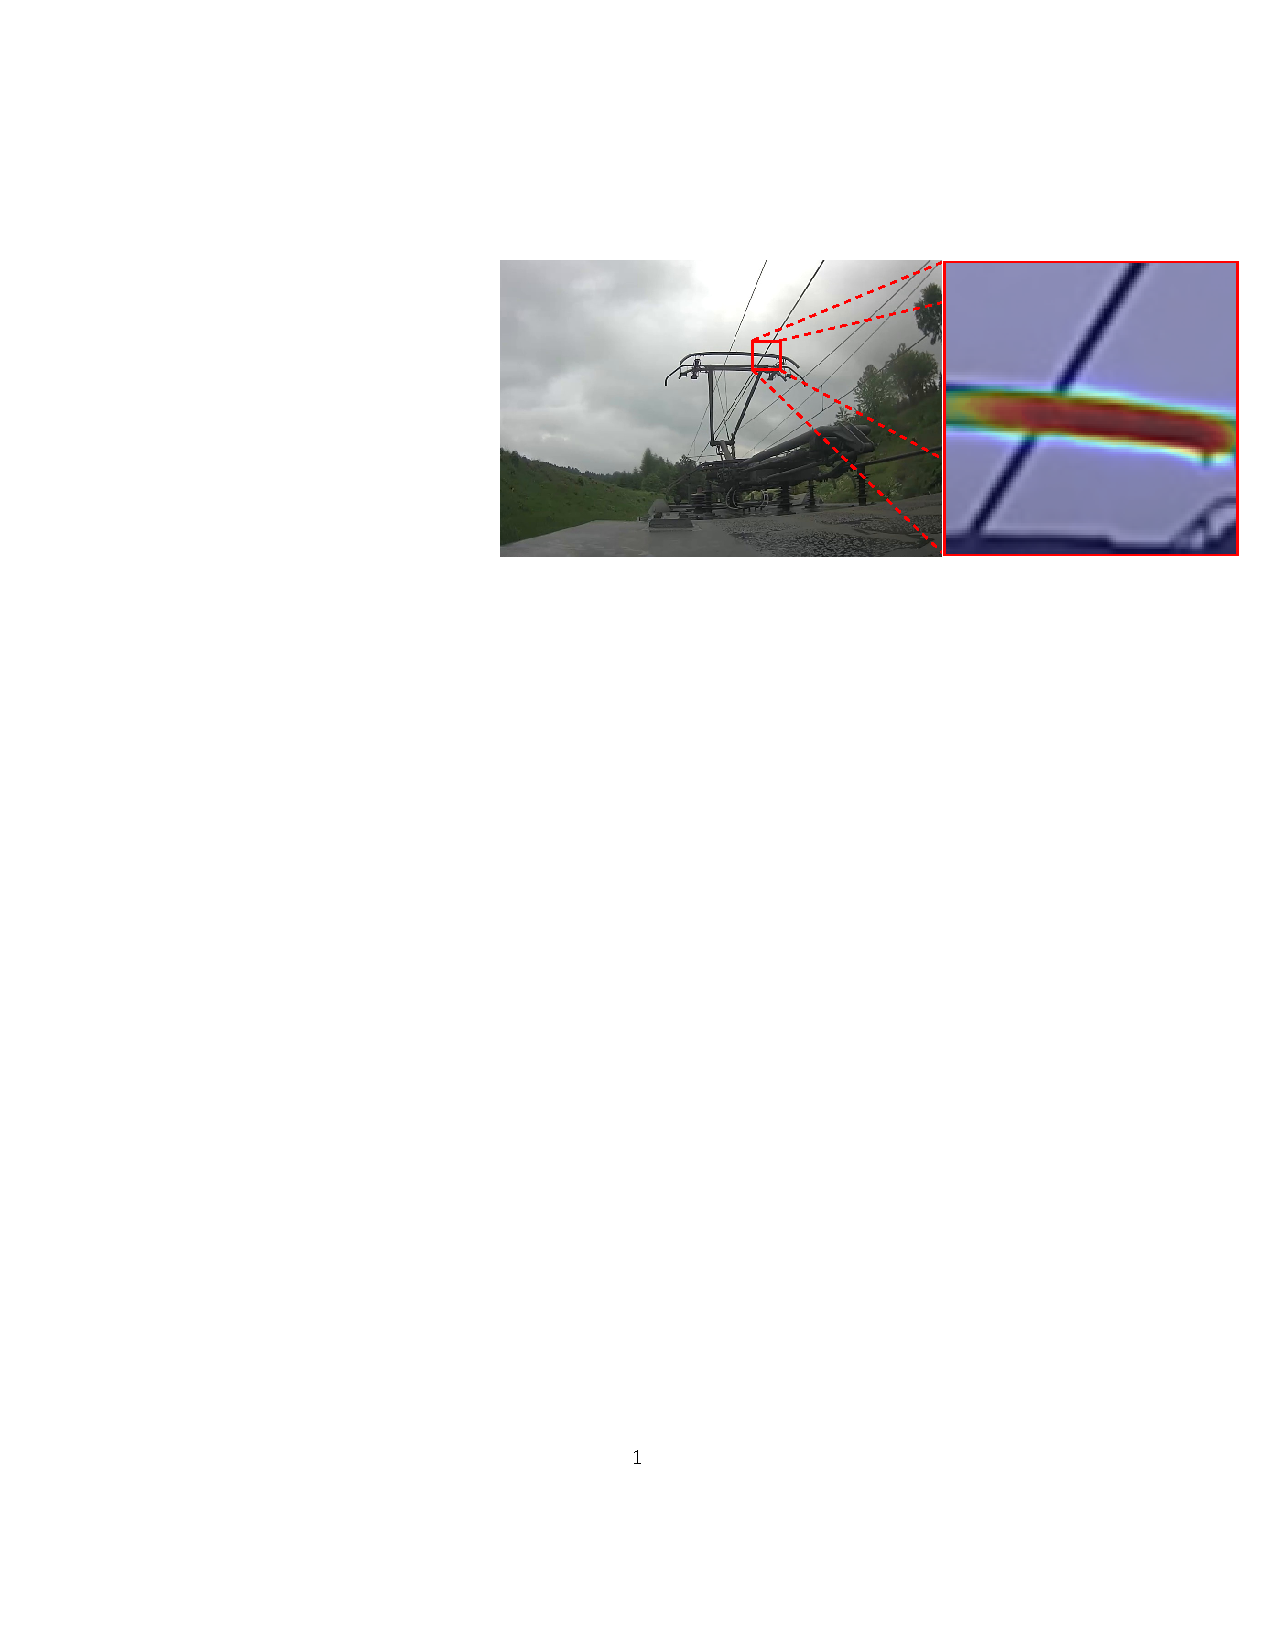
\includegraphics[trim={10cm 18.5cm 0.5cm 4.3cm},clip,height = 1in]{img/fail/merge}
\\


\end{tabular}

\caption{Failure cases: motion blur and ``non-object'' instance.}
\label{fig:fail}
\vspace{-0.2cm}
\end{figure}

\mypar{Failure cases.}
Finally, we discuss two scenarios in which SiamMask fails: motion blur and ``non-object'' instance (Figure~\ref{fig:fail}).
Despite being different in nature, these two cases arguably arise from the complete lack of similar training samples in a training sets, which are focused on objects that can be unambiguously discriminated from the foreground.
